\documentclass[12pt,letterpaper]{article}
\usepackage[utf8]{inputenx} %Codificacion del texto (ISO Latin1 encoding)

\usepackage{fancyhdr} %Permite acomodar a tu gusto la parte de arriba y
% abajo del documento
\usepackage[spanish]{babel} %Permite definir el idioma del dcumento
\usepackage{graphicx} %Permite exportar imagenes en formato eps
\usepackage{url} %Tipo de fuente para correos y paginas
\usepackage{pgf}
\usepackage{fleqn}
\usepackage{amssymb}
\usepackage{amsmath}
\usepackage{fancyvrb}
\usepackage{makeidx}
\usepackage{colortbl} %Permite colocar colores a las tablas
\usepackage{multirow}
\usepackage{booktabs}
\usepackage{moreverb}
\usepackage{rotating}
\usepackage[final]{pdfpages}
%%%%%%%%%%
%Margenes%
%%%%%%%%%%
\parskip 1mm %Espacio entre parrafos

\setlength{\topmargin}{0pt}
\topmargin      0.5cm
\oddsidemargin	0.1cm  % Ancho Letter 21,59cm
\evensidemargin 0.5cm  % Alto  Letter 27,81cm
\textwidth	17cm%15.5cm
\textheight	21.0cm
\headsep	4 mm
\parindent	0.5cm
%%%%%%%%%%%%%%%%%%%%%%
%Estilo del documento%
%%%%%%%%%%%%%%%%%%%%%%
\pagestyle{fancyplain}

%%%%%%%%%%%%%%%%%%%%%%%%%%%%%%%%%%%%%%%%%%%
%Fancyheadings. Top y Bottom del documento%
%%%%%%%%%%%%%%%%%%%%%%%%%%%%%%%%%%%%%%%%%%%
% Recuerde que en este documento la portada del documento no posee
% numeracion, pero de igual manera llamaremos a esa primera pagina la numero
% 1, y la que viene la dos. Esto es para tener una idea de las que
% llamaremos pares e impares
\lhead{Laboratorio mat023} %Parte superior izquierda
\rhead{\bf \it Preinforme 1} %Parte superior derecha
\lfoot{\it } %Parte inferior izquierda. \thepage indica
% el numero de pagina
\cfoot{} %Parte inferior central
\rfoot{\bf \thepage} %Parte inferior derecha
\renewcommand{\footrulewidth}{0.4pt} %Linea de separacion inferior

\newcommand{\primaria}[1]{
	\textbf{\underline{#1}}
}

\newcommand{\foranea}[1]{
	\textbf{\textsl{#1}}
}

\newcommand{\primyfor}[1]{
	\underline{\foranea{#1}}
}

\makeatletter
\newcommand\subsubsubsection{\@startsection {paragraph}{1}{\z@}%
                                   {-3.5ex \@plus -1ex \@minus -.2ex}%
                                   {1.5ex \@plus.2ex}%
                                   {\normalfont\bfseries}}
\newcommand\subsubsubsubsection{\@startsection {subparagraph}{1}{\z@}%
                                   {-3.5ex \@plus -1ex \@minus -.2ex}%
                                   {1.5ex \@plus.2ex}%
                                   {\normalfont\bfseries}}


\makeatother
 

\begin{document}
\title{Laboratorio mat023 \\ \begin{Large}Preinforme 1\end{Large}} 
\author{Victor Gonzalez Rodriguez\\victor.gonzalezro@alumnos.usm.cl\\2773029-9}
\date{\today}
\maketitle

\section{Problema}

Existe un sistema de estanques en una planta de tratamiento de hormigón por donde fluyen mezclas de cemento y agua. Inicialmente en el estanque 1, contiene 100\textbf{k} litros de mezcla en la que se han disuelto 40 kilos de cemento. En el estanque 2, con 500 litros de capacidad, contiene 200 litros de mezcla con una concentración de $1/20$ kilos de cemento por litro.
\\

En el instante $t = 0$ se abren simultáneamente las válvulas A, B, C y D para iniciar el flujo de mezclas.
Por A entra mezcla con concentración de $1/25$ kilos de cemento por litro a 25 litros por minuto. Por B pasa la mezcla del tanque 1 hacia el tanque 2 a 25 litros por minuto. Por C entra agua pura a \textbf{n} litros por minuto y por D sale mezcla a \textbf{m} litros por minuto.
\\

Considere que las mezclas son perfectas y que no existe adherencia de cemento en las paredes de los
estanques y en las tuberías de flujo

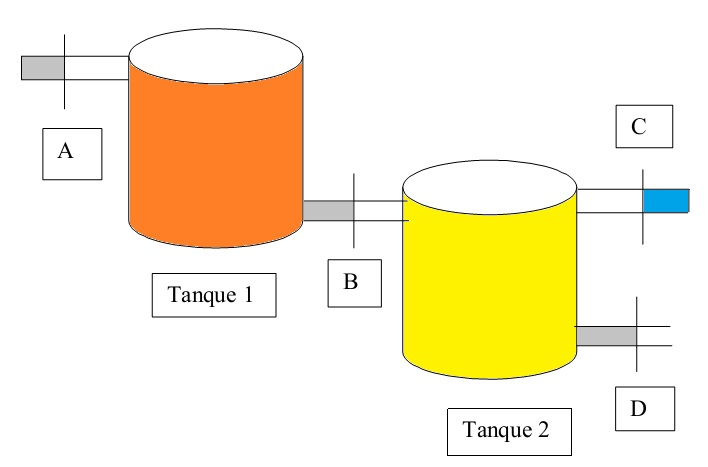
\includegraphics[width=\textwidth]{modelo.png}



\section{Solución}
\subsection{Variables del problema}

Para los problemas que se entregan a continuación se deben usar las siguientes constantes:
\begin{description}
\item[k:] penúltimo dígito no nulo de su rol = 9
\item[m:] su bloque horario = 2
\item[n:] día de la semana que tiene laboratorio = 2
\end{description}

Por lo tanto:
\begin{description}
\item[Flujo de entrada C:] $2 [\frac{lt}{min}]$
\item[Flujo de salida D:] $2 [\frac{lt}{min}]$
\item[Volumen estanque 1:] $900 [lt]$
\end{description}

\newpage

\subsection{Cantidad neta de cemento en el estanque 1}

\begin{center}
$C_1(t) := $ Cantidad de cemento del estanque 1 en el instante $t$.
\end{center}

Teniendo en cuenta la situación que nos pone el problema, podemos identificar que existe una cierta cantidad de cemento que está entrando por A, y que está saliendo por B en un instante cualquiera. Es por esto que podemos definir un diferencial de la cantidad de cemento ilustrada de la siguiente manera:

\begin{center}
$\dfrac{dC_1}{dt} = \dfrac{cemento\ entrante}{tiempo} - \dfrac{cemento\ saliente}{tiempo}$ (1)
\end{center}

Sea $A_f$ el flujo de entrada de la tubería A, $A_c$ la concentración de la mezcla entrante por A, $B_f$ el flujo de salida de la tubería B, y $B_c$ la concentración de la mezcla saliente por B. Entonces, la ecuación en (1) quedaría como:

\begin{center}
$\dfrac{dC_1}{dt} = A_c[\frac{Kg}{lt}]A_f[\frac{lt}{min}] - B_c[\frac{Kg}{lt}]B_f[\frac{lt}{min}]$
\end{center}
\begin{center}
$\dfrac{dC_1}{dt} = \dfrac{1}{25}[\frac{Kg}{lt}]25[\frac{lt}{min}] - \dfrac{C_1(t)}{900 + flujo\ neto*t}[\frac{Kg}{lt}]25[\frac{lt}{min}]$
\end{center}

Aquí podemos notar, que el flujo neto que ingresa al estanque 1, es 0, ya que los $25 [\frac{lt}{min}]$ que entran en A, se anulan con los $25 [\frac{lt}{min}]$ que salen por B. Entonces

\begin{center}
$\dfrac{dC_1}{dt} =1[\frac{Kg}{min}] - \dfrac{C_1(t)}{36}[\frac{Kg}{min}]$
\end{center}

Nos hemos encontrado con una ecuación diferencial lineal de primer grado. Al resolver esta ecuación, obtenemos que:

\begin{center}
$C_1(t) = k e^{-\frac{t}{36}}+36$, donde $k\in\mathbb{R}$
\end{center}

Y como sabemos que en $t=0$ hay $40[Kg]$ de cemento, podemos encontrar $k$. Finalmente, la ecuación para la cantidad neta de cemento en el estanque 1 es: 

\begin{center}
$C_1(t) = 4 e^{-\frac{t}{36}}+36$
\end{center}

\subsection{Instante $t_1$ en el que se llena el estanque 2}

Esto puede ser facilmente calculado tomando el flujo que entra por B, por C y que sale por D. Por lo tanto, para saber como se va llendando el estanque, debemos calcular el flujo neto.\\

Por B está entrando $25 [\frac{lt}{min}]$, por C está entrando $2 [\frac{lt}{min}]$ y por D está saliendo $2 [\frac{lt}{min}]$, por lo que el flujo neto, es simplemente $25 [\frac{lt}{min}]$.

Dado que en $t_0 = 0$ hay $200 [lt]$ en el estanque, la ecuación de volumen que nos permitirá encontrar $t_1$ es:

\begin{center}
$V(t) = 25t+200$
\end{center}

Entonces, cuando $V(t_1)=500$:
\begin{center}
$V(t_1) = 500 = 25t_1+200$
\end{center}
\begin{center}
$t_1=\dfrac{300}{25}=12$
\end{center}

Por lo tanto, a los 12 minutos, el estanque 2 quedará completamente lleno.
\end{document}